\subsection{Tra RTB e PB}
\subsubsection{Settimo periodo  01/02/2024 - 16/02/2024}
\paragraph{Considerazioni}
Durante il settimo periodo, si è svolta la prima parte della revisione RTB con il Prof. Cardin, il cui esito è stato positivo, ottenendo il semaforo verde. \\
In seguito alla revisione, il professore ha segnalato alcuni punti critici riguardanti l'\textit{Analisi dei Requisiti}, per la quale sono già state eseguite delle attività correttive. \\
Per quanto riguarda il PoC, sono emerse possibili problematiche gestionali non affrontate sulla modalità di comunicazione tra Kafka e ClickHouse. A tal proposito, si è tenuta una riunione con il proponente al fine di elaborare una soluzione valida. Tale soluzione, in breve, prevede la rimozione dell'intermediario da noi gestito e l'istituzione di una connessione diretta tra Kafka e ClickHouse tramite strumenti robusti (ulteriori dettagli sono riportati nel verbale esterno datato 09/02/2024). \\
Durante questo periodo, quindi, è stata sviluppata dai programmatori la soluzione individuata. Oltre a ciò, il \textit{Responsabile} ha condotto le attività necessarie per organizzare e richiedere la seconda parte della revisione con il Professore Vardanega. \\
In conclusione, tra le attività pianificate, è stata deliberata l'allocazione di risorse per la fase iniziale della progettazione del diagramma delle classi relativa alla simulazione dei sensori, nonostante sia stato chiarito nel più recente diario di bordo che il focus del progetto non è su questo specifico ambito. Tuttavia, in accordo con il proponente, si è deciso di progettare anche questo segmento di prodotto rispettando le regole ed identificando i design pattern adeguati così da fare esperienza.
   
\paragraph{Gestione dei rischi} 

\begin{itemize}
    \item \textbf{Rischi attesi e verificati:}
\begin{itemize}
    \item \textbf{RO-2M-2} - Ritardo nel completamento delle attività rispetto ai tempi previsti (\ref{sec:ritAttivita})
    \begin{itemize}
        \item \textbf{Esito mitigazione:} 
        Per evitare prolungamenti nel periodo stabilito e considerando la disponibilità di alcuni membri, il \textit{Responsabile} ha deciso di riassegnare alcune attività. \\
        L'esito è risultato soddisfacente poiché tutte le attività programmate sono state completate.
        \item \textbf{Impatto:}
        L'arrivo degli esiti degli esami ha provocato imprevedibili necessità di ulteriore studio per alcuni membri, i quali avevano già delle attività assegnate. Questa problematica ha comportato un leggero ritardo nell'esecuzione di alcune di tali attività, che sono state quindi riassegnate ad altri membri liberi dagli esami. Ciò ha generato un leggero sovraccarico, tuttavia tutte le attività pianificate per il periodo sono state completate.
    \end{itemize}
\end{itemize}
\item \textbf{Rischi attesi ma non verificati:}
 \begin{itemize}
    \item  \textbf{RT-1A-1 -} Apprendimento ed utilizzo delle nuove tecnologie (\textit{\ref{sec:rischioTec}}): dovuto alla necessità di una nuova modalità di comunicazione tra Kafka e ClickHouse.
\end{itemize}
\item \textbf{Rischi non attesi ma verificati:}
\begin{itemize}
    \item Nessuno.
\end{itemize}
\end{itemize}

\paragraph{Definizione ruoli}
Per le \textit{attività}\textsubscript{\textit{G}} registrate nei costi, sono stati assegnati i seguenti ruoli: 

\vspace{0.4cm}

\begin{table}[H]
    \centering
    \begin{tabular}{|L{4cm}|L{2cm}|}
        \hline
        \textbf{Ruolo} & \textbf{Persona} \\
        \hline
        \hline
        Responsabile (Re)   & A. Barutta \\
        \hline
        Amministratore (Am) & E. Hysa \\
        \hline
        Analisti (An)       & E. Hysa \\
                            & N. Preto \\
        \hline
        Verificatore (Ve)   & A. Barutta \\
                            & F. Pozza \\
        \hline
        Programmatori (Pr)  & D. Diotto\\
                            & L. Skenderi \\
        \hline
        Progettista (Pt)    & R. Smanio \\
                            & D. Diotto \\
        \hline
    \end{tabular}
    \caption{Tabella dei Ruoli e delle Persone - settimo periodo}
    \label{tab:Ruoli_persone_7}
    \end{table}

\newpage
\paragraph{Pianificazione attività divise per ruoli con consuntivo e preventivo orario e dei costi}

\vspace{0.4cm}

\begin{figure}[H]
    \centering
    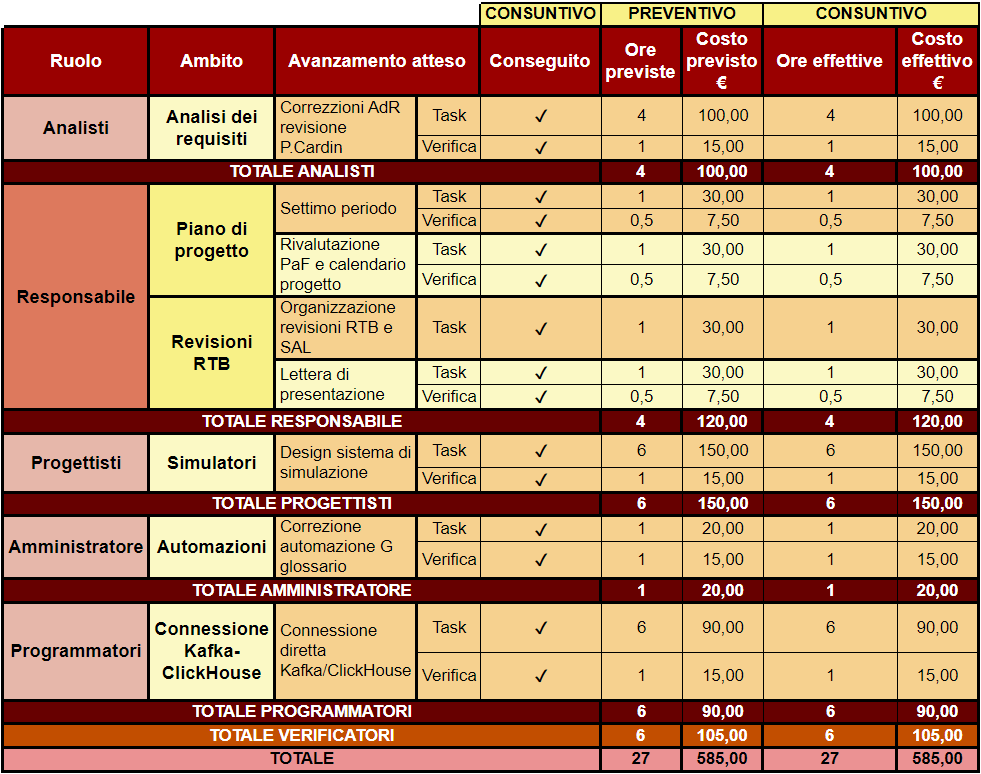
\includegraphics[height=0.9\textwidth]{../Images/periodo7.PNG}
    \caption{Settimo periodo}
    \label{fig:Settimo_periodo}
\end{figure}


Al termine del settimo periodo, l'ammontare totale del costo del progetto è \textbf{ 4592,50\euro\ } e sono state completate il \textbf{100\%} delle \textit{attività}\textsubscript{\textit{G}} attese.
Il preventivo a finire rimane invariato a \textbf{12425,00€}.
In accordo con il proponente, si è deciso di ridurre la durata di ciascun periodo ad una settimana, con conseguente adeguamento dei SAL, considerando la maggiore disponibilità oraria del gruppo a seguito della conclusione delle lezioni e della sessione di esami invernale.
\href{https://github.com/orgs/ByteOps-swe/projects/3/views/1?sortedBy%5Bdirection%5D=asc&sortedBy%5BcolumnId%5D=64182560}{Vai al Diagramma di Gantt.}

\pagebreak

\paragraph{Preventivo orario}

\begin{figure}[H] 
    \centering
    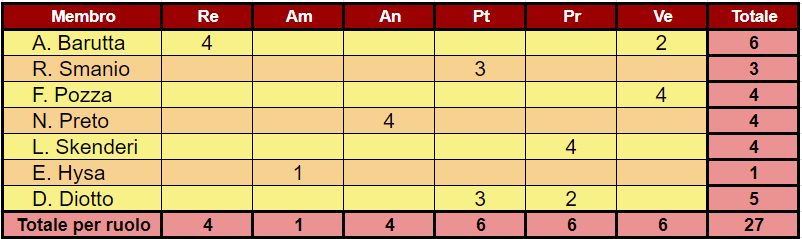
\includegraphics[width=0.9\textwidth]{../Images/preventivoOrario7Periodo.png}
    \caption{Preventivo orario per membro - settimo periodo}
    \label{fig:Preventivo_orario_7}
\end{figure}

\vspace{0.6cm}

\begin{figure}[H]
    \centering
    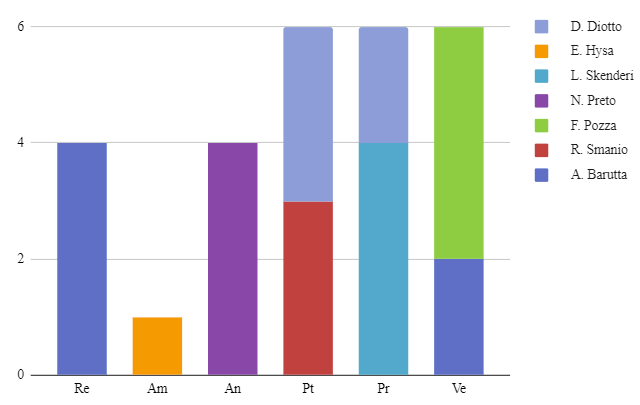
\includegraphics[width=0.6\textwidth]{../Images/preventivoDivisioneRuoli7Periodo.png}
    \caption{Istogramma preventivo della ripartizione oraria dei ruoli - settimo periodo}
    \label{fig:Preventivo_ripartizione_oraria_7}
\end{figure}

\pagebreak

\paragraph{Consuntivo orario}

\begin{figure}[H]
    \centering
    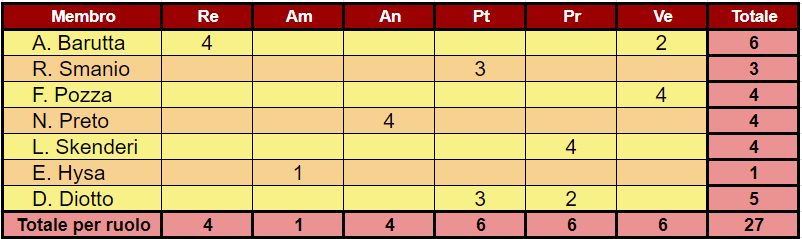
\includegraphics[width=0.9\textwidth]{../Images/consuntivoOrario7Periodo.png}
    \caption{Consuntivo orario per membro - settimo periodo}
    \label{fig:Constuntivo_orario_7}
\end{figure}

\vspace{0.6cm}

\begin{figure}[H]
    \centering
    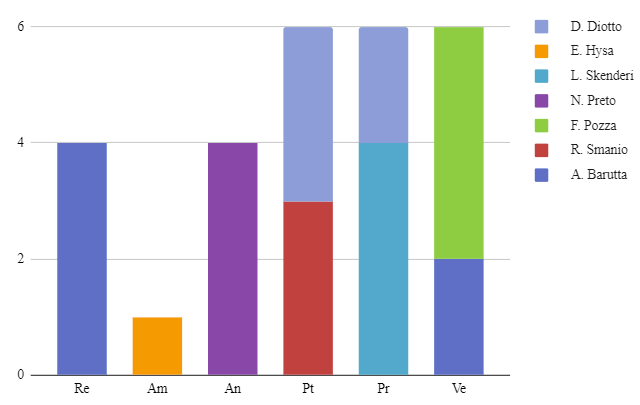
\includegraphics[width=0.6\textwidth]{../Images/consuntivoDivisioneRuoli7Periodo.png}
    \caption{Istogramma consuntivo della ripartizione oraria dei ruoli - settimo periodo}
    \label{fig:Consuntivo_ripartizione_oraria_7}
\end{figure}
